%% ****** Start of file apstemplate.tex ****** %
%%
%%   This file is part of the APS files in the REVTeX 4 distribution.
%%   Version 4.1r of REVTeX, August 2010
%%
%%
%%   Copyright (c) 2001, 2009, 2010 The American Physical Society.
%%
%%   See the REVTeX 4 README file for restrictions and more information.
%%
%
% This is a template for producing manuscripts for use with REVTEX 4.0
% Copy this file to another name and then work on that file.
% That way, you always have this original template file to use.
%
% Group addresses by affiliation; use superscriptaddress for long
% author lists, or if there are many overlapping affiliations.
% For Phys. Rev. appearance, change preprint to twocolumn.
% Choose pra, prb, prc, prd, pre, prl, prstab, prstper, or rmp for journal
%  Add 'draft' option to mark overfull boxes with black boxes
%  Add 'showpacs' option to make PACS codes appear
%  Add 'showkeys' option to make keywords appear
\documentclass[10pt,%
               aps,%
               prl,%
               preprint,%
               superscriptaddress,%
               preprintnumbers,%
               amsmath,%
               floatfix,%
               endfloats*]{revtex4-2}
\usepackage[T1]{fontenc}
\usepackage[utf8x]{inputenc} 
\usepackage[export]{adjustbox}  % Used to adjust figure frames
\usepackage{subcaption}
\usepackage{url}
\usepackage{color}
\usepackage{xcolor}
\usepackage{listings}
\usepackage{float}
\usepackage{amsfonts}
\usepackage{wrapfig}
\usepackage{physics}
\usepackage{mathtools}  % For shortintertext
\usepackage[inline]{enumitem}
\usepackage[per-mode=symbol,group-separator={,},group-minimum-digits=4]{siunitx}
\usepackage{todonotes}
\usepackage{graphicx}
\graphicspath{ {../paper_figures} }
\usepackage{bibentry}

%%% HELPER CODE FOR DEALING WITH EXTERNAL REFERENCES
\usepackage{xr-hyper}
\usepackage[pdftex,%
            colorlinks=true,%
            linkcolor=blue,%
            citecolor=blue,%
            urlcolor=blue,%
            bookmarksnumbered=true,%
            bookmarksopen=true]{hyperref}
\usepackage[capitalize]{cleveref}
\makeatletter
\newcommand*{\addFileDependency}[1]{
  \typeout{(#1)}
  \@addtofilelist{#1}
  \IfFileExists{#1}{}{\typeout{No file #1.}}
}
\makeatother

\newcommand*{\myexternaldocument}[2][ext:]{
    \externaldocument[#1]{#2}
    \addFileDependency{#2.tex}
    \addFileDependency{#2.aux}
}
%%% END HELPER CODE

% put all the external documents here!
\myexternaldocument[main:]{paper}

\begin{document}

\title{Supplemental Material: Multidimensional analysis and detection of informative features in human white matter}
  
\author{Adam \surname{Richie-Halford}}%
\email{richford@uw.edu}%
\affiliation{%
    eScience Institute,%
    University of Washington, Seattle,%
    Washington 98195--1560, USA
}
  
\author{Jason \surname{Yeatman}}%
\affiliation{%
    Graduate School of Education and Division of Developmental and Behavioral Pediatrics,%
    Stanford University,%
    Stanford, CA, 94305, USA
}

\author{Noah \surname{Simon}}%
\affiliation{%
    Department of Biostatistics,%
    University of Washington, Seattle,%
    Washington 98195--1560, USA
}

\author{Ariel \surname{Rokem}}%
\affiliation{%
    Department of Psychology,%
    University of Washington, Seattle,%
    Washington 98195--1560, USA
}

\date{\today}

\preprint{NT@UW-20-21}
%\pacs{}
\begin{abstract}
In these supplemental materials we present\ldots
\end{abstract}

\maketitle

\makeatletter
\def\l@subsubsection#1#2{}
\makeatother
\tableofcontents

%\newpage
\section{Online Methods}
\label{sec:methods}

\subsection{Data}
\label{sec:data}

Four different previously-published datasets were used here:

\begin{enumerate}

\item Diffusion MRI from a previous study of the corticospinal
tract (CST) in patients with amyotrophic lateral sclerosis
(ALS \cite{sarica2017corticospinal}), containing data from 24 ALS
patients and 24 demographically matched healthy controls. These data
were measured in a GE Discovery 750 3T MRI scanner at the Institute
of Bioimaging and Molecular Physiology in Catanzaro. Informed consent
was provided as approved by the Ethical Committee of the University
``Magna Graecia'' of Catanzaro. Voxel resolution was \num{2x2x2}
$\text{mm}^3$ and 27 non-colinear directions were measured with a
$b=1000$ $\frac{\text{sec}}{\text{mm}^2}$. Data was preprocessed to 
correct for subject motion and for eddy currents. The diffusion tensor
model \cite{basser1994mr} was fit in every voxel.
We will refer to this dataset as ALS.

\item Diffusion MRI data from a previous study of properties of
the white matter across the lifespan \cite{yeatman2014lifespan},
containing dMRI data from 76 subjects with ages 6-50. These data were
measured in a GE Discovery 750 3T MRI scanner at the Stanford Center
for Cognitive and Neurobiological Imaging. The Stanford University
IRB approved the procedures of this study. Informed consent was
obtained from each adult participant, and assent for participation
was provided by parents/guardians for children. Voxel resolution was
\num{2x2x2}$\text{mm}^3$ with 96 non-colinear directions measured with a
$b=2000$ $\frac{\text{sec}}{\text{mm}^2}$ and 30 non-colinear directions
measured with a $b=1000$ $\frac{\text{sec}}{\text{mm}^2}$. These data
were acquired using a dual spin echo sequence, in which there is
sufficient time for eddy currents to subside between the application of
the gradients and the image acquisition, so no eddy current correction
was applied, but motion correction was applied before fitting the
diffusion tensor model \cite{basser1994mr} in every voxel using a robust
fit \cite{chang2005restore}. We will refer to this dataset as WH.

\item Diffusion MRI data from the Healthy Brain Network pediatric mental
health study \cite{alexander2017open}, containing dMRI data from 978 subjects
with ages 5-21. These data were measured in 3T Siemens MRI scanners at three
sites in the New York area. Informed consent was obtained from each
participant aged 18 or older. For participants younger than 18, written
consent was obtained from their legal guardians and written assent was
obtained from the participant. Voxel resolution was
\num{1.8x1.8x1.8}$\text{mm}^3$ with 64 non-colinear directions measured for
each of $b=1000 \frac{\text{sec}}{\text{mm}^2}$ and $b=2000
\frac{\text{sec}}{\text{mm}^2}$.
Preprocessing was performed using \emph{QSIPrep} 0.12.1, which is based on
\emph{Nipype} 1.5.1 \cite[RRID:SCR\_002502]{nipype1,nipype2}.

\begin{itemize}

\item {\it Anatomical data preprocessing}
The T1-weighted (T1w) image was corrected for intensity non-uniformity
(INU) using \texttt{N4BiasFieldCorrection} \cite[ANTs 2.3.1]{n4}, and
used as T1w-reference throughout the workflow. The T1w-reference was
then skull-stripped using \texttt{antsBrainExtraction.sh} (ANTs 2.3.1),
using OASIS as target template. Spatial normalization to the ICBM 152
Nonlinear Asymmetrical template version 2009c
\cite[RRID:SCR\_008796]{mni} was performed through nonlinear
registration with \texttt{antsRegistration} \cite[ANTs 2.3.1,
RRID:SCR\_004757]{ants}, using brain-extracted versions of both T1w
volume and template. Brain tissue segmentation of cerebrospinal fluid
(CSF), white-matter (WM) and gray-matter (GM) was performed on the
brain-extracted T1w using \texttt{FAST} \cite[FSL 6.0.3:b862cdd5,
RRID:SCR\_002823]{fsl_fast}.

\item {\it Diffusion data preprocessing}
Several confounding time-series were calculated based on the
\emph{preprocessed DWI}: framewise displacement (FD) using the
implementation in \emph{Nipype} \cite[following the definitions
by]{power_fd_dvars}. The head-motion estimates calculated in the
correction step were also placed within the corresponding confounds
file. Slicewise cross correlation was also calculated. The DWI
time-series were resampled to ACPC, generating a \emph{preprocessed DWI
run in ACPC space}.
\end{itemize}

Many internal operations of \emph{QSIPrep} use \emph{Nilearn} 0.6.2
\cite[RRID:SCR\_001362]{nilearn} and \emph{Dipy} \cite{dipy}. For more
details of the pipeline, see
\href{https://qsiprep.readthedocs.io/en/latest/workflows.html}{the
section corresponding to workflows in \emph{QSIPrep}'s documentation}.
We will refer to this dataset as HBN.

\item Diffusion MRI data from the Cambridge Centre for Ageing and
Neuroscience (Cam-CAN) ``CC700'' dataset
\cite{shafto2014cambridge,taylor2017cambridge}, containing data from 640
subjects with ages 18-88. These data were measured on a 3T Siemens TIM Trio
system and written informed consent was obtained from each participant. Voxel
resolution was \num{2x2x2}$\text{mm}^3$ with 30 non-colinear directions
measured for each of $b=1000$ $\frac{\text{sec}}{\text{mm}^2}$ and $b=2000$
$\frac{\text{sec}}{\text{mm}^2}$. The diffusion weighted images were acquired
with a twice refocused spin-echo sequence and the same preprocessing pipeline
used for the HBN dataset was applied to this data. We will refer to this
dataset as Cam-CAN.

\end{enumerate}

Data from the ALS and WH studies was processed in a similar manner,
using the Matlab Automated Fiber Quantification toolbox (\texttt{mAFQ})
\cite{yeatman2012tract}: streamlines representing fascicles of white
matter tracts were generated using a determinstic tractography algorithm
that follows the prinicpal diffusion direction of the diffusion tensor
in each voxel (STT) \cite{basser2000vivo}. Major tracts were identified
using multiple criteria: streamlines are selected as candidates for
inclusion in a bundle of streamlines that represents a tract if they
pass through known inclusion ROIs and do not pass through exclusion
ROIs \cite{wakana2007reproducibility}. In addition, a probabilistic
atlas is used to exclude streamlines which are unlikely to be part of
a tract \cite{Hua2008-sh}. Each streamline is resampled to 100 nodes
and the robust mean at each location is calculated by estimating the 3D
covariance of the location of each node and excluding streamlines that
are more than 5 standard deviations from the mean location in any node.
Finally, a bundle profile of tissue properties in each bundle was created
by interpolating the value of MRI maps of these tissue properties to the
location of the nodes of the resampled streamlines designated to each
bundle. In each of 100 nodes, the values are summed across streamlines,
weighting the contribution of each streamline by the inverse of the
mahalnobis distance of the node from the average of that node across
streamlines. This means that streamlines that are more representative of
the tract contribute more to the bundle profile, relative to streamlines
that are on the edge of the tract.

Data from the HBN and Cam-CAN studies were processed using the updated
Python Automated Fiber Quantification toolbox (\texttt{pyAFQ}).
\todo[inline]{Add pyAFQ citation} In addition to demonstrating the our
analysis pipeline is robust to changes in the platform and version number of
tractometry software, the use of the updated \texttt{pyAFQ} capitalized upon
the following three improvements over the legacy Matlab version
\begin{enumerate*}[%
    label=(\roman*),%
    before=\unskip{: },%
    itemjoin={{, }},%
    itemjoin*={{, and }}]
    \item the ability to ingest data provided in the BIDS format
    \cite{gorgolewski2016brain}
    \item the calculation of diffusion kertosis imaging (DKI
    \cite{jensen2005diffusion}) metrics
    \item the exclusion of the Cingulum Hippocampus bundles, which
    demonstrated low reliability in the legacy \texttt{mAFQ}.
\end{enumerate*}
We will refer to the \texttt{mAFQ} and \texttt{pyAFQ} pipeline collectively
as \texttt{AFQ}.

These processes create bundle profiles, in which diffusion measures
are quantified and averaged along twenty major fiber tracts. Here,
we use only the mean diffusivity (MD) and the fractional anisotropy
(FA) of the diffusion tensor, but additional dMRI-based maps or maps
based on other quantitative MRI measurements can also be used. These
bundle profiles, along with the phenotypical data we wish to explain
or predict, form the input to the SGL algorithm. In a domain-agnostic
machine learning context, the phenotypical data comprise the target
variables while the bundle profiles form the feature or predictor
variables (See \cref{main:fig:methods:group-structure} in the main text).

\subsection{Sparse Group Lasso}

Before fitting a model to the data, imputation and standardization are
performed. Missing node values (e.g., in cases where \texttt{AFQ} designates
a node as not-a-number) are imputed via linear interpolation. Care is taken
not to interpolate across the boundaries between different bundles. Some
diffusion metrics will have naturally larger variance than others and may
therefore dominate the objective function and make the SGL estimator unable
to learn from the lower variance metrics. For example, fractional anisotropy
(FA) is bounded between zero and one and could be overwhelmed by an unscaled
higher-variance metric like the mean diffusivity (MD). To prevent this we
remove each feature's mean and scale it to unit variance (z-score) using the
\lstinline{StandardScaler} from scikit-learn \cite{scikit-learn}. The scaling
parameters are learned only from the training data and then applied equally
to the training and test data in order to prevent leakage of information
between the testing and training sets \cite{kaufman2012leakage}.

After scaling and imputation, the tractometry data and target
phenotypical data can be organized in a linear model:
\begin{equation}
    y = \mathbf{X} \beta + \epsilon,
    \label{eq:lm}
\end{equation}
where $y$ is the phenotype -- categorical, such as a clinical diagnosis,
or continuous numerical, such as the subject's age. The tractometry
data is represented in the feature matrix $\mathbf{X}$, with rows
corresponding to different subjects, and columns corresponding
to diffusion measures at different nodes within each bundle. The
relationship between tractometric features and the phenotypic target is
characterized by the coefficients in $\beta$. The error term, $\epsilon$
is an unobserved random variable that captures the error in the model.
We denote our prediction of the targer phenotype as $\hat{y}$ and the
coefficients that produce this prediction as $\hat{\beta}$, so that
\begin{equation}
    \hat{y} = \mathbf{X} \hat{\beta},
    \label{eq:lm-approx}
\end{equation}
without the error term, $\epsilon$. In general, the feature matrix
$\mathbf{X}$ has dimensions $S \times (B \times N \times M)$, where $S$
is the number of subjects, $B$ is the number of white matter bundles,
$N$ is the number of nodes in each bundle, and $M$ is the number of
diffusion metrics calculated at each node. Typically, $B = 20$, $N =
100$, and $2 \le M \le 8$, resulting in $\sim 4,000 - 16,000$ features.
Conversely, many dMRI studies have between a few dozen and a few
hundred subjects, yielding a feature matrix that is wide and short.
Even in cases where more than a thousand subjects are measured (e.g.,
in the Human Connectome Project, where 1,200 subjects were measured
\cite{VanEssen2012}), the problem is ill-posed: the high dimensionality
of this data requires regularization to avoid overfitting and generate
interpretable results.

Here, we propose that in addition to regularizing the coefficients in
$\hat{\beta}$, we can also capitalize on our knowledge of the group structure
of the bundle profile features in $\mathbf{X}$. The bundle-metric
combinations form a natural grouping. For example, we expect that MD features
within the left arcuate fasciculus will co-vary across individuals. Likewise
for FA values within the right corticospinal tract (CST) and so on. This
group structure is represented in \cref{main:fig:methods:group-structure}, which
depicts the linear model $\hat{y} = \mathbf{X} \hat{\beta}$. Thus, we seek a
regularization approach that will fit a linear model with
anatomically-grouped covariates, where we expect to observe both groupwise
sparsity, where the number of groups (bundle/metric combinations) with at
least one non-zero coefficients is small, as well as within-group sparsity,
where the number of non-zero coefficients within each non-zero group is
small. The sparse group lasso (SGL) is a penalized regression technique that
satisfies exactly these criteria\cite{simon2013sparse}. It solves for a
coefficient vector $\hat{\beta}$ that satisfies
\begin{multline}
    \hat{\beta} = \min_\beta L_{\text{mse}}
    + \left( 1 - \alpha \right) \lambda \displaystyle \sum_{\ell = 1}^{G}
    \sqrt{p_\ell} \norm{\beta^{(\ell)}}_2
    + \alpha \lambda \norm{\beta}_1,\\%
    \text{where} \quad
    L_{\text{mse}} = \frac{1}{2}
    \norm{y - \displaystyle \sum_{\ell = 1}^{G}
    \mathbf{X}^{(\ell)} \beta^{(\ell)}}_2^2
    \label{eq:sgl}
\end{multline}
where $G$ is the number of groups $\mathbf{X}^{(\ell)}$ is the submatrix of
$\mathbf{X}$ corresponding to group $\ell$, $\beta^{(\ell)}$ is the
coefficient vector for group $\ell$ and $p_\ell$ is the length of
$\beta^{(\ell)}$. In the tractomtetry setting, $G = T \times M$ and $\forall
\ell: p_\ell = 100$. The first term is the mean square error loss,
$L_{\text{mse}}$, as in the standard linear regression framework. The second
and third terms encourage groupwise sparsity and overall sparsity,
respectively. If $\alpha = 1$ the SGL reduces to the traditional
lasso\cite{tibshirani1996regression}. Conversely, if $\alpha = 0$ the SGL
reduces to the group lasso\cite{yuan2006model}. Thus, the model
hyperparameter $\alpha$ controls the combination of group-lasso and lasso.
The hyperparameter $\lambda$ controls the strength of the regularization.

\subsubsection{Incorporating target transformations}

Often, the target variable $y$ is not in the domain in which the linear
model can be best fit to it. \Cref{eq:lm-approx} can be slightly
modified as:
\begin{equation}
    \hat{y} = f^{-1} \left( \mathbf{X} \hat{\beta} \right),
    \label{eq:lm-transform}
\end{equation}
where the transformation function $f^{-1}$ characterizes the transform
applied to the data before fitting the linear coefficients. For example,
For the WH, HBN, and Cam-CAN datasets, we use a logarithmic transform,
\begin{equation}
    f \left( \hat{y} \right) = \ln \left( \hat{y} \right)
    \label{eq:log-nonlinearity}
\end{equation}

\subsubsection{Classification of categorical targets}
When the phenotypical target variable is categorical, as in the case of
explaining or predicting the presence of a clinical diagnosis, the SGL is
readily adapted to logistic regression, where the probability of a target
variable belonging to an arbitrary defined ``true'' class is the logistic
function of the result of the linear model,
\begin{equation}
    p(\hat{y} = 1) = \frac{1}{1 + \exp(\mathbf{X} \hat{\beta})},
    \label{eq:logit}
\end{equation}
or equivalently, the mean squared error loss function in \cref{eq:sgl} is
replaced with the cross-entropy loss, which for binary classification is the
negative log likelihood of the SGL classifier giving the ``true'' label:
\begin{equation}
    L_{\text{mse}} \rightarrow L_{\log} =
    -\left(y \log(p) + (1 - y) \log(1 - p)\right).
    \label{eq:logloss}
\end{equation}

\subsection{Implementation, cross-validation and metaparameter optimization}

Because the SGL is not specific to tractometry, we implement its solution as
a separate Python package called \texttt{groupyr} \cite{groupyr}.
\texttt{Groupyr} solves the cost function in \cref{eq:sgl} using proximal
gradient descent \cite{parikh2014proximal} by implementing a custom proximal
operator and relying on the C-OPT optimization library \cite{copt}, providing
a fitted SGL model as a scikit-learn compatible estimator \cite{sklearn_api}.
\texttt{Groupyr} also selects the hyperparameters $\alpha$ and $\lambda$ that
yield the best cross-validated performance using either
\begin{enumerate*}[%
    label=(\roman*),%
    before=\unskip{: },%
    itemjoin={{, }},%
    itemjoin*={{, or }}]
    \item an exhaustive grid search of hyperparameter combinations
    \item sequential model based optimization using the scikit-optimize
    library \cite{scikit_optimize}.
\end{enumerate*}

\todo[inline]{%
    Rewrite the remainder of this section to reflect \texttt{groupyr} changes.
}

To objectively evaluate the model performance and guard against over-fitting,
we used a nested cross-validation scheme, depicted in
\cref{main:fig:methods:cross-val} for the categorical classification case.
The subjects (i.e. rows of the feature matrix $\mathbf{X}$ in
\cref{main:fig:methods:group-structure} and \cref{eq:lm}) are shuffled and
then decomposed into $k$ batches, hereafter referred to as folds. For
the ALS dataset we used $k=10$ and for the WH dataset $k=5$. For each
unique fold, we hold that fold out as the test\textsubscript{outer} set
and let the remaining data comprise the train\textsubscript{outer} set,
with the subscript indicating the depth of the nested decomposition.
We further decompose each train\textsubscript{outer} set into three
folds, and again for each unique fold, we hold out that fold as the
test\textsubscript{inner} set and let the remaining data comprise the
train\textsubscript{inner} set. At level-1 of the decomposition, we fit
an SGL model using fixed regularization meta-parameters $\alpha$
and $\lambda$, training the model using train\textsubscript{inner}
and evaluating the fit on test\textsubscript{inner}. We find
the optimal values for $\alpha$ and $\lambda$ using
hyperoptimization, implemented using the hyperopt library's \verb|fmin|
function\cite{Bergstra_2015} with a tree of Parzen estimators search
algorithm\cite{bergstra2011algorithms}. For continuous numerical $y$,
\verb|fmin| searches for meta-parameter values that minimize the median
absolute error. This can also be done minimizing the root of the mean
squared error (RMSE) or to maximizing the coefficient of determination
($R^2$). For binary categorical $y$ \verb|fmin| seeks to maximize the
classification accuracy. This can also be done maximizing the area
under the receiver operating curve (ROC AUC) or the average precision.
Using hyperoptimization, we find optimal regularization parameters and
$\hat{\beta}$ for each train\textsubscript{outer} set and then use those
to predict values for data in test\textsubscript{outer}. Thus each
subject in the dataset has a predicted phenotype derived from a model
that never saw its particular subject's data.

The above procedure describes $k$-fold cross validation. In fact, we use
repeated $k$-fold cross validation on the outer level of the decomposition, so
that the input data is decomposed into $k$ folds, three times. Thus, each
subject has three predicted phenotypes. We then take the mean predicted value to
summarize the performance of the model. In the classification case, the
shuffling into folds is stratified such that each fold has a population that
preserves the percentage of each class found in the larger input data.

\subsection{Software implementation}

The full software implementation of the SGL approach presented here is available
in a Python software package called AFQ-Insight, which is developed publicly in
\url{https://github.com/richford/afq-insight}. The version of the code used to
produce the results herein is also available in
\url{https://doi.org/10.5281/zenodo.3585942}.
\todo[inline]{Update version here}
AFQ-Insight reads the target and feature data that has been processed by AFQ
from comma separated value (CSV) files conforming to the AFQ-Browser data
format \cite{yeatman2018browser} and represents them internally as
\lstinline{DataFrame} objects from the pandas Python
library \cite{mckinney2010data}. The software provides different options for
imputing missing data in the feature matrix. Missing interior nodes are imputed
using linear interpolation. For missing exterior nodes, the user may choose
between linear extrapolation and constant forward(back)-fill. Imputation uses
only values from adjacent nodes in the same white matter bundle in the same
subject so there is no danger of data leakage from other subjects. It uses the
scikit-learn \cite{scikit-learn} library to decompose input data into separate
test and train datasets, to scale each feature to have zero mean and
unit variance, and to evaluate each fit in the hyperparameter search using
appropriate classification and regression metrics such as accuracy, area
under the receiver operating curve (AUC ROC), and coefficient of determination
($R^2$). For each set of hyperparameters, we solve the SGL using a custom
proximal operator supplied to the C-OPT library\cite{copt}. Appropriate
hyperparameters are found using the hyperopt library\cite{Bergstra_2015}.

\section{Bundle and coefficient profiles}
\label{sec:bundle-profiles}

Here, we present the bundle profiles and $\hat{\beta}$ coefficients
for each dataset. Throughout this section, diffusion metrics are plotted
along the length of eighteen bundles: 
right corticospinal (CST\_R),
left corticospinal (CST\_L),
right uncinate (UNC\_R),
left uncinate (UNC\_L),
left inferior fronto-occipital fasciculus (IFO\_L),
right inferior fronto-occipital fasciculus (IFO\_R),
right arcuate (ARC\_R),
left arcuate (ARC\_L),
right thalamic radiation (ATR\_R),
left thalamic radiation (ATR\_L),
right cingulum cingulate (CGC\_R),
left cingulum cingulate (CGC\_L),
callosum forceps major (FP),
callosum forceps minor (FA),
right inferior longitudinal fasciculus (ILF\_R),
left inferior longitudinal fasciculus (ILF\_L),
right superior longitudinal fasciculus (SLF\_R),
and left superior longitudinal fasciculus (SLF\_L).
We display results for two different diffusion metrics: fractional anisotropy
(fa) and mean diffusivity (md). We use lower-case letters to abbreviate the
diffusion metrics and distinguish fractional anisotropy (fa) from the
callosum forceps minor (FA).

\subsection{ALS bundle profiles}

\begin{figure*}
    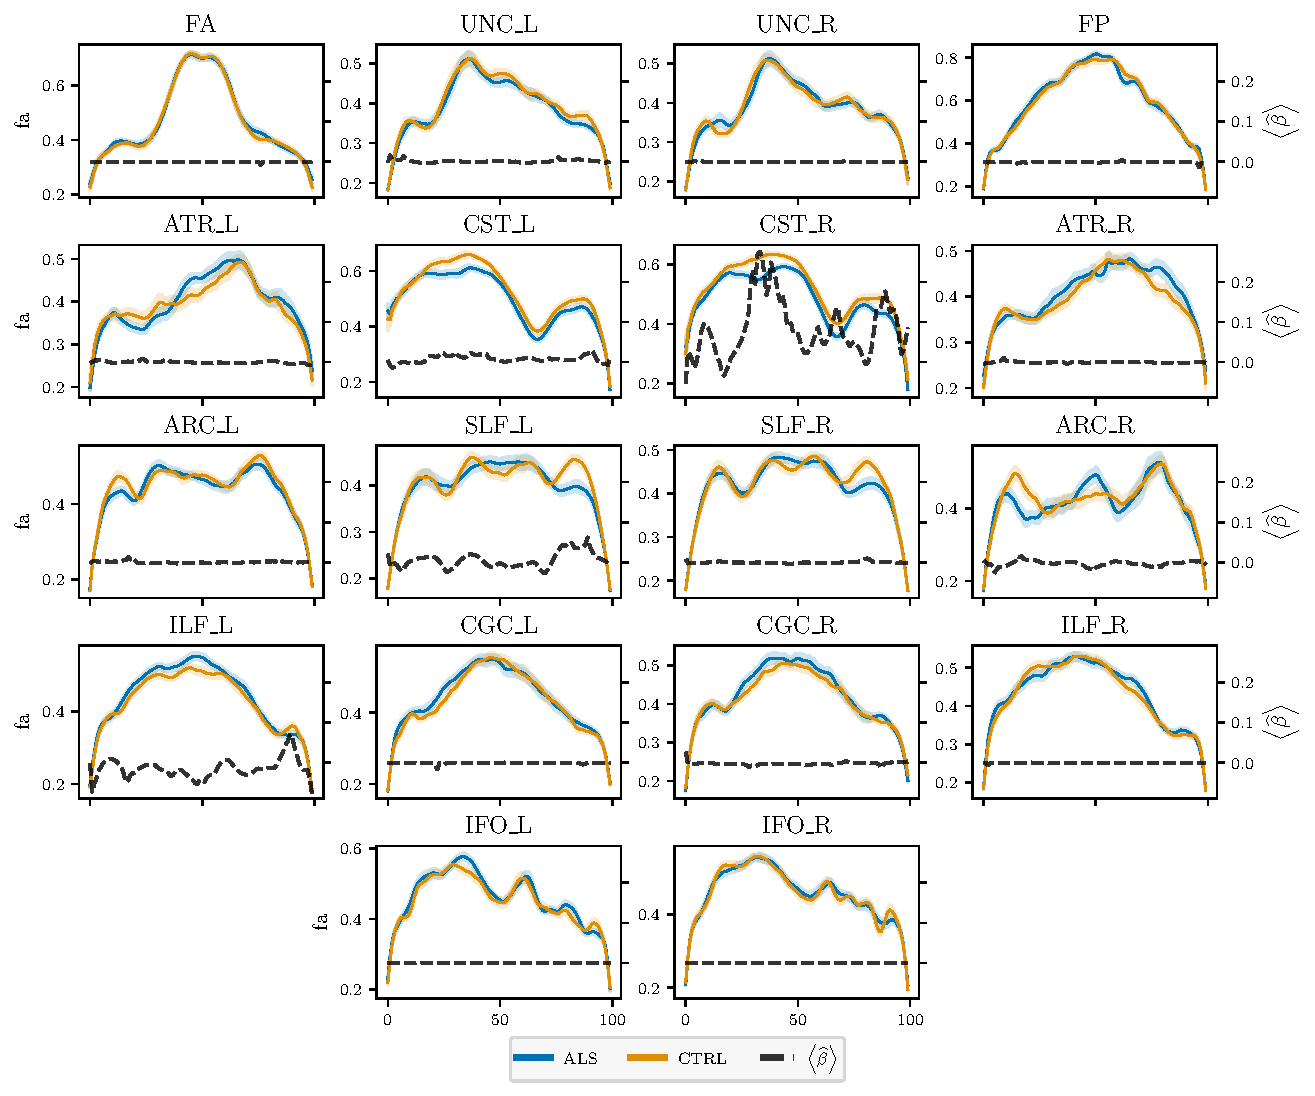
\includegraphics[width=\textwidth]{sarica_coefs_profiles_fa.pdf}
    \caption{%
        {%
            \bf Fractional anisotropy (fa) bundle profiles and $\hat{\beta}$
            coefficients for ALS classification.
        }
        \label{fig:als-bp:fa}
    }
\end{figure*}

\Cref{fig:als-bp:fa,fig:als-bp:md} show the bundle profiles and regression
coefficients for the ALS dataset fa and md metrics, respectively. The scale
of the $\hat{\beta}$ axes is shared between the fa and md figures to
highlight the relative importance of the fa features over the md features.

\begin{figure*}
    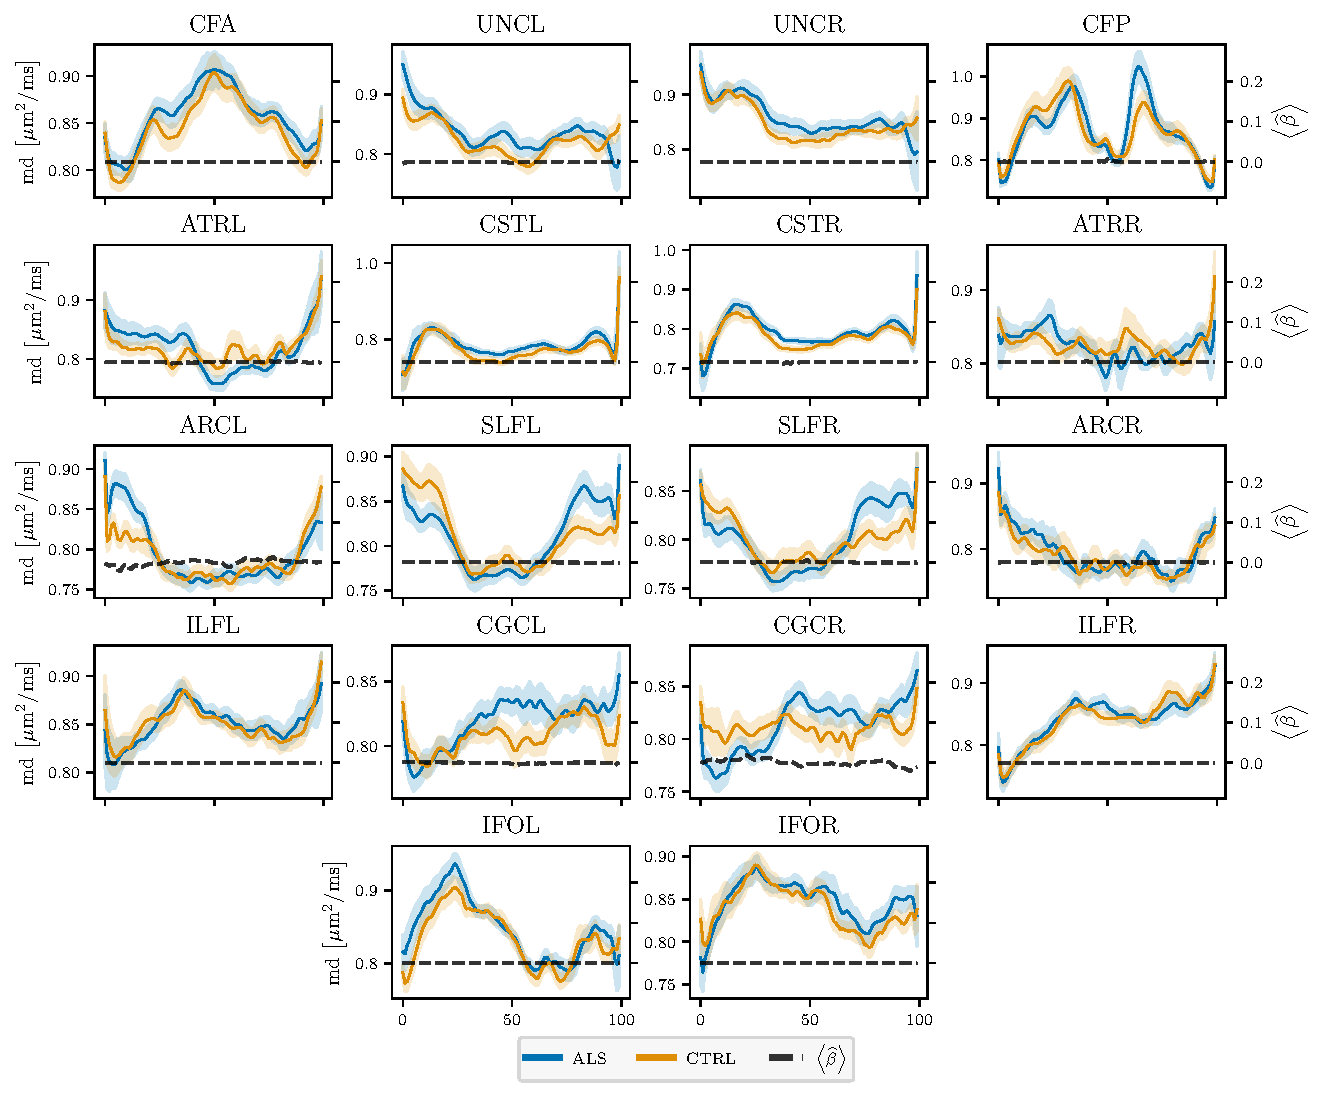
\includegraphics[width=\textwidth]{sarica_coefs_profiles_md.pdf}
    \caption{%
        {%
            \bf Mean diffusivity (md) Bundle profiles and $\hat{\beta}$
            coefficients for ALS classification.
        }
        \label{fig:als-bp:md}
    }
\end{figure*}

\subsection{WH bundle profiles}

\begin{figure*}
    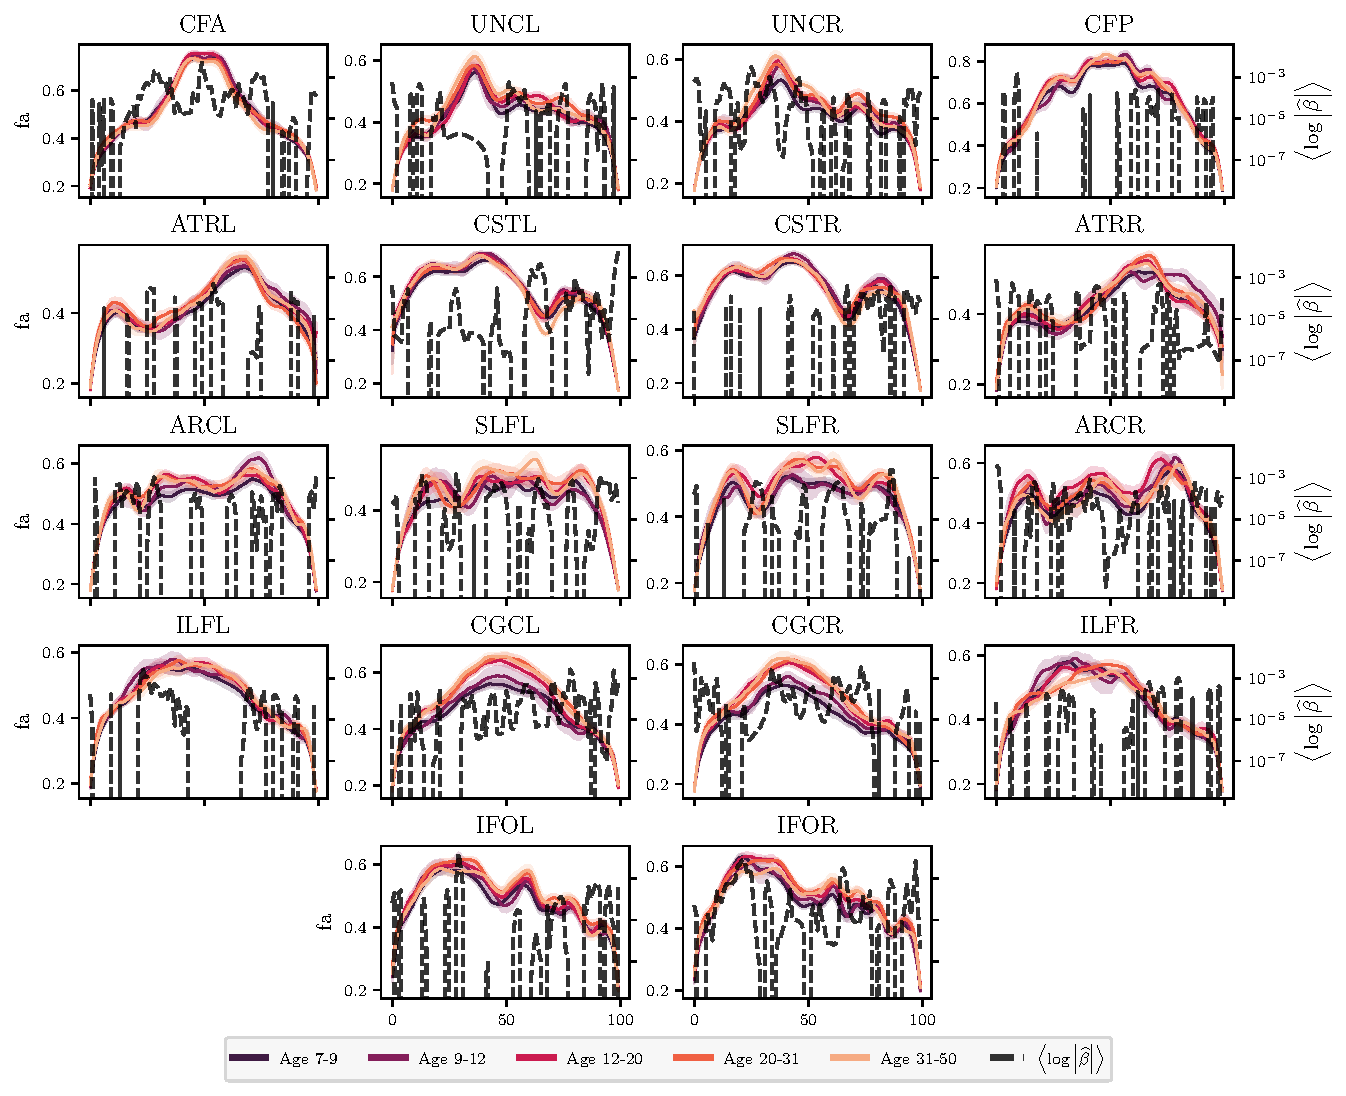
\includegraphics[width=\textwidth]{wh_coefs_profiles_fa.pdf}
    \caption{%
        {%
            \bf Fractional anisotropy (fa) bundle profiles and $\hat{\beta}$
            coefficients for age regression in the WH dataset.
        }
        \label{fig:wh-bp:fa}
    }
\end{figure*}

\hspace{1em}

\begin{figure*}
    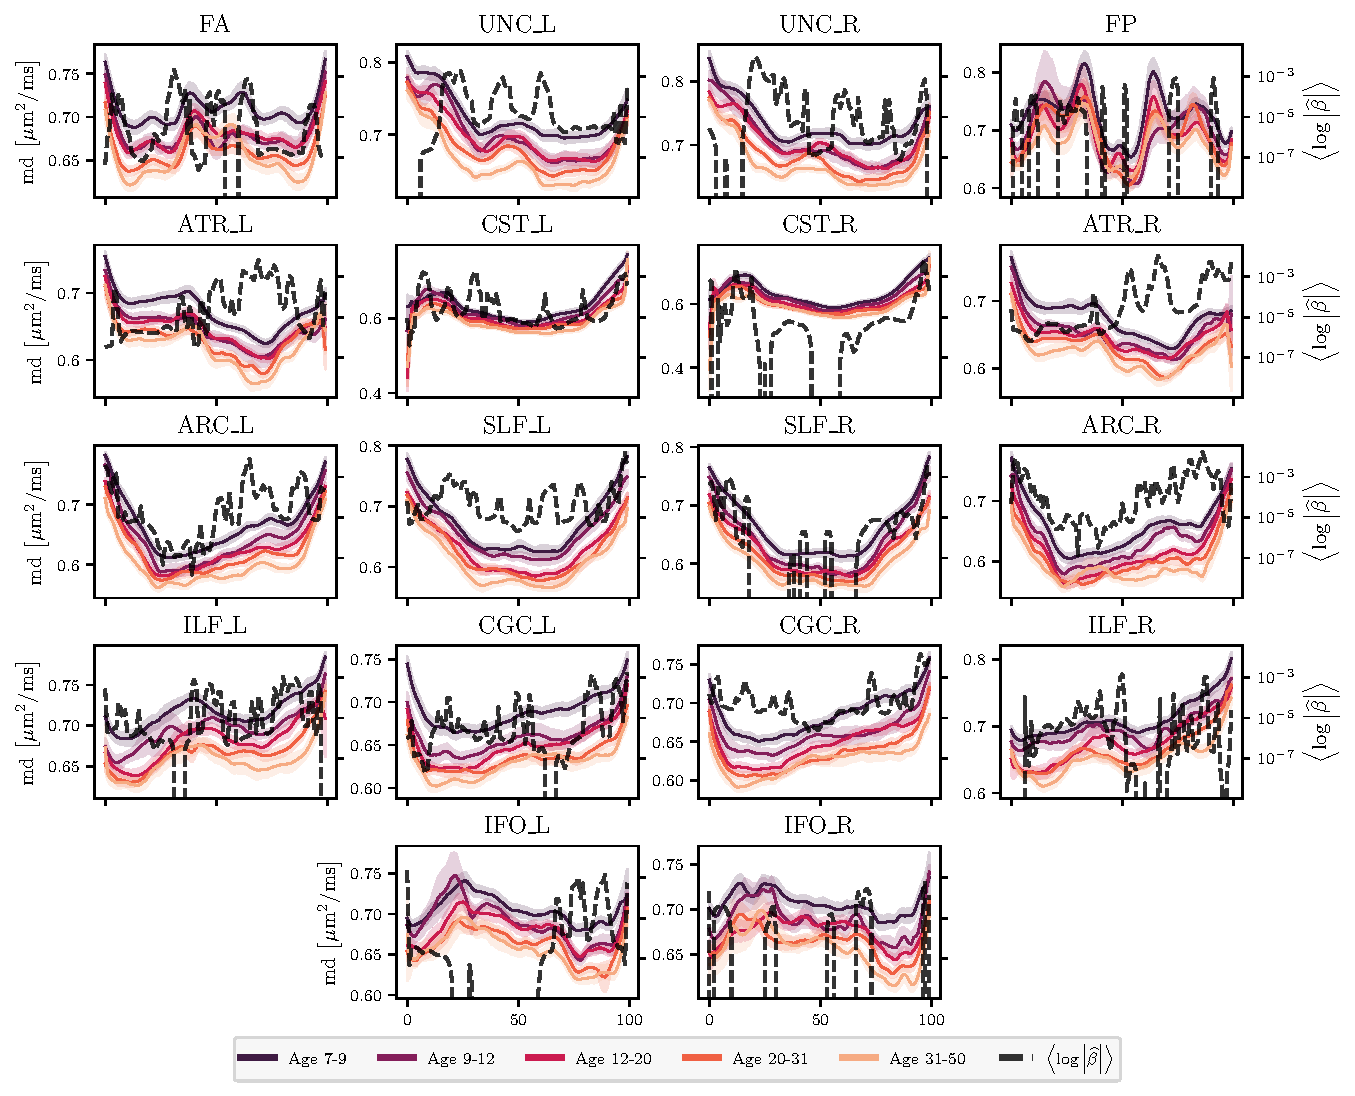
\includegraphics[width=\textwidth]{wh_coefs_profiles_md.pdf}
    \caption{%
        {%
            \bf Mean diffusivity (md) bundle profiles and $\hat{\beta}$
            coefficients for age regression in the WH dataset.
        }
        \label{fig:wh-bp:md}
    }
\end{figure*}

\subsection{HBN bundle profiles}

\begin{figure*}
    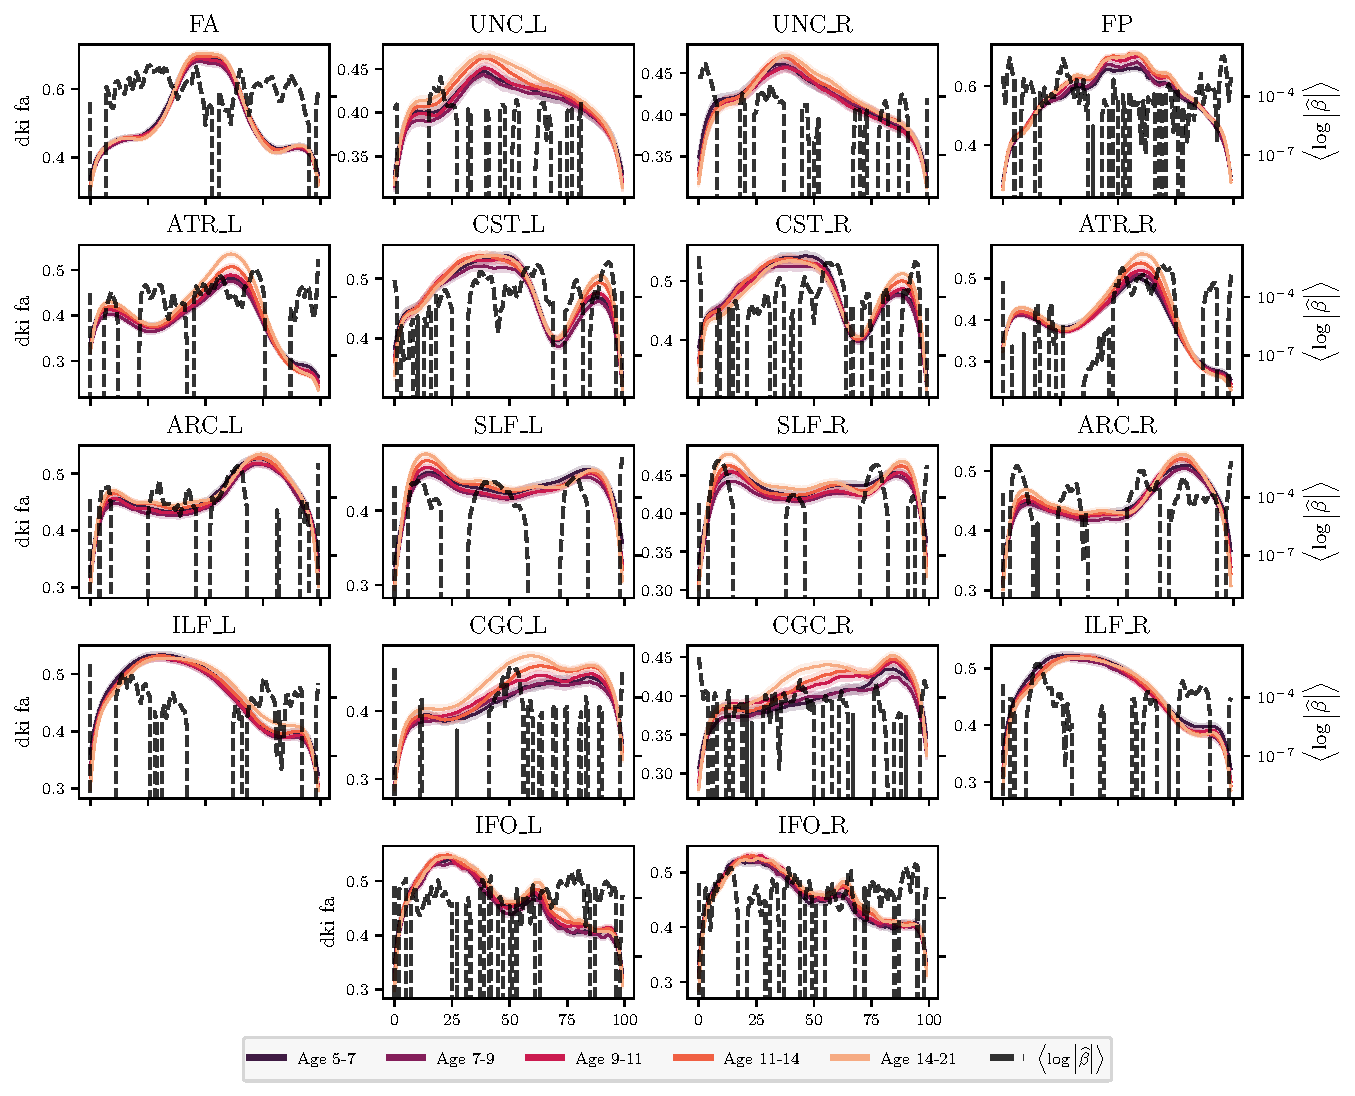
\includegraphics[width=\textwidth]{hbn_coefs_profiles_fa.pdf}
    \caption{%
        {%
            \bf Fractional anisotropy (fa) bundle profiles and $\hat{\beta}$
            coefficients for age regression in the HBN dataset.
        }
        \label{fig:hbn-bp:fa}
    }
\end{figure*}

\hspace{1em}

\begin{figure*}
    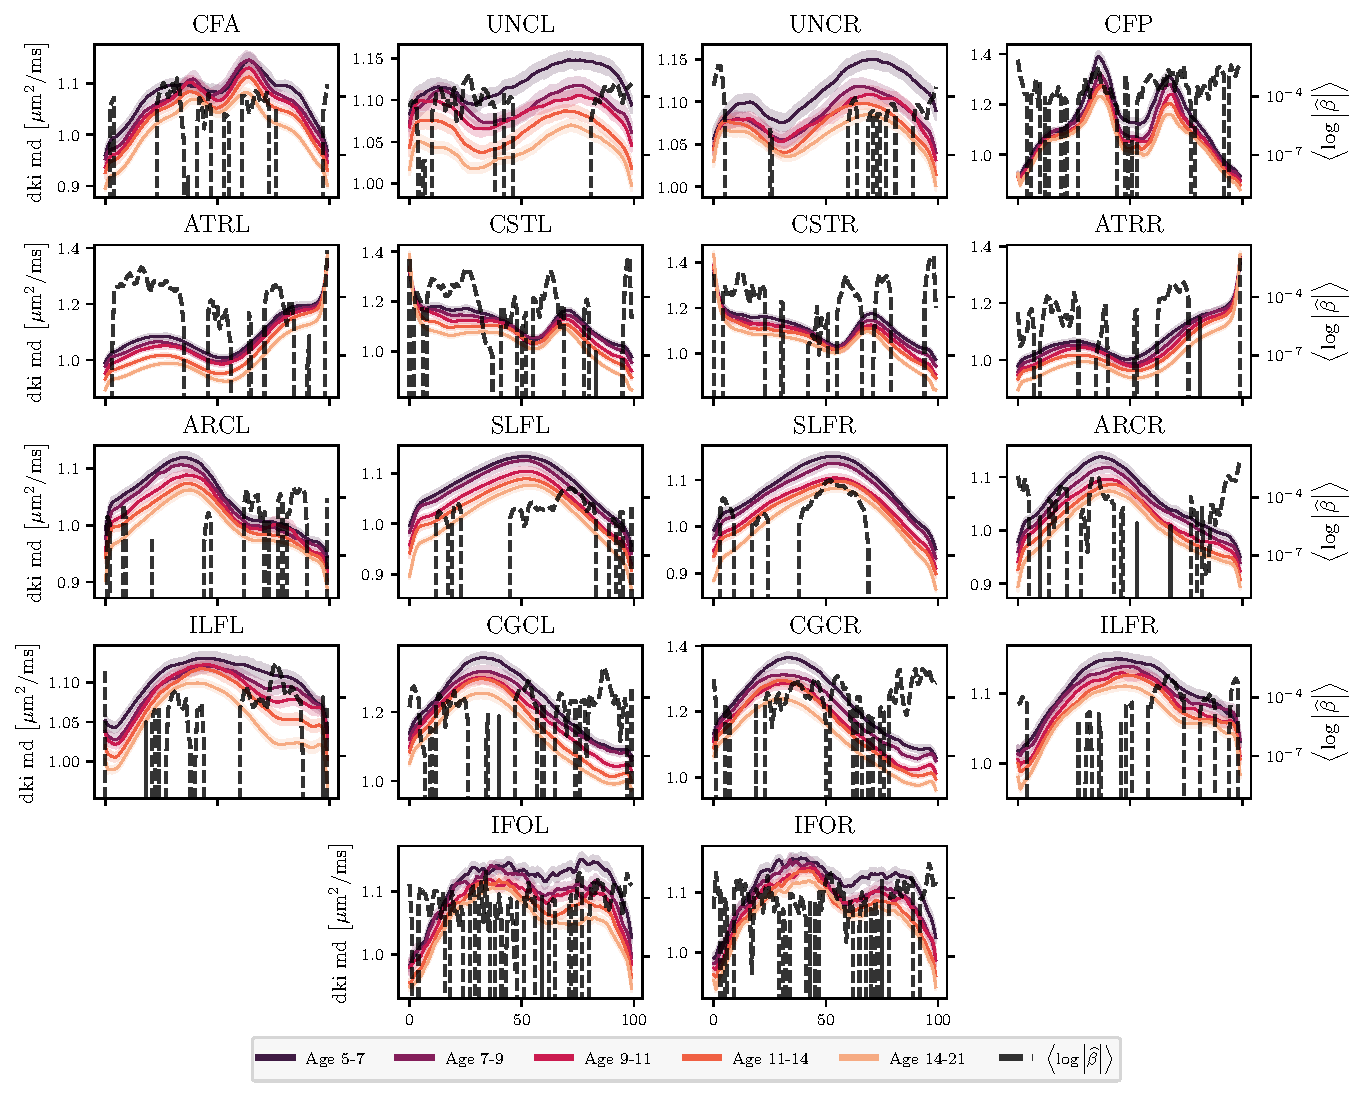
\includegraphics[width=\textwidth]{hbn_coefs_profiles_md.pdf}
    \caption{%
        {%
            \bf Mean diffusivity (md) bundle profiles and $\hat{\beta}$
            coefficients for age regression in the HBN dataset.
        }
        \label{fig:hbn-bp:md}
    }
\end{figure*}

\subsection{Cam-CAN bundle profiles}

\begin{figure*}
    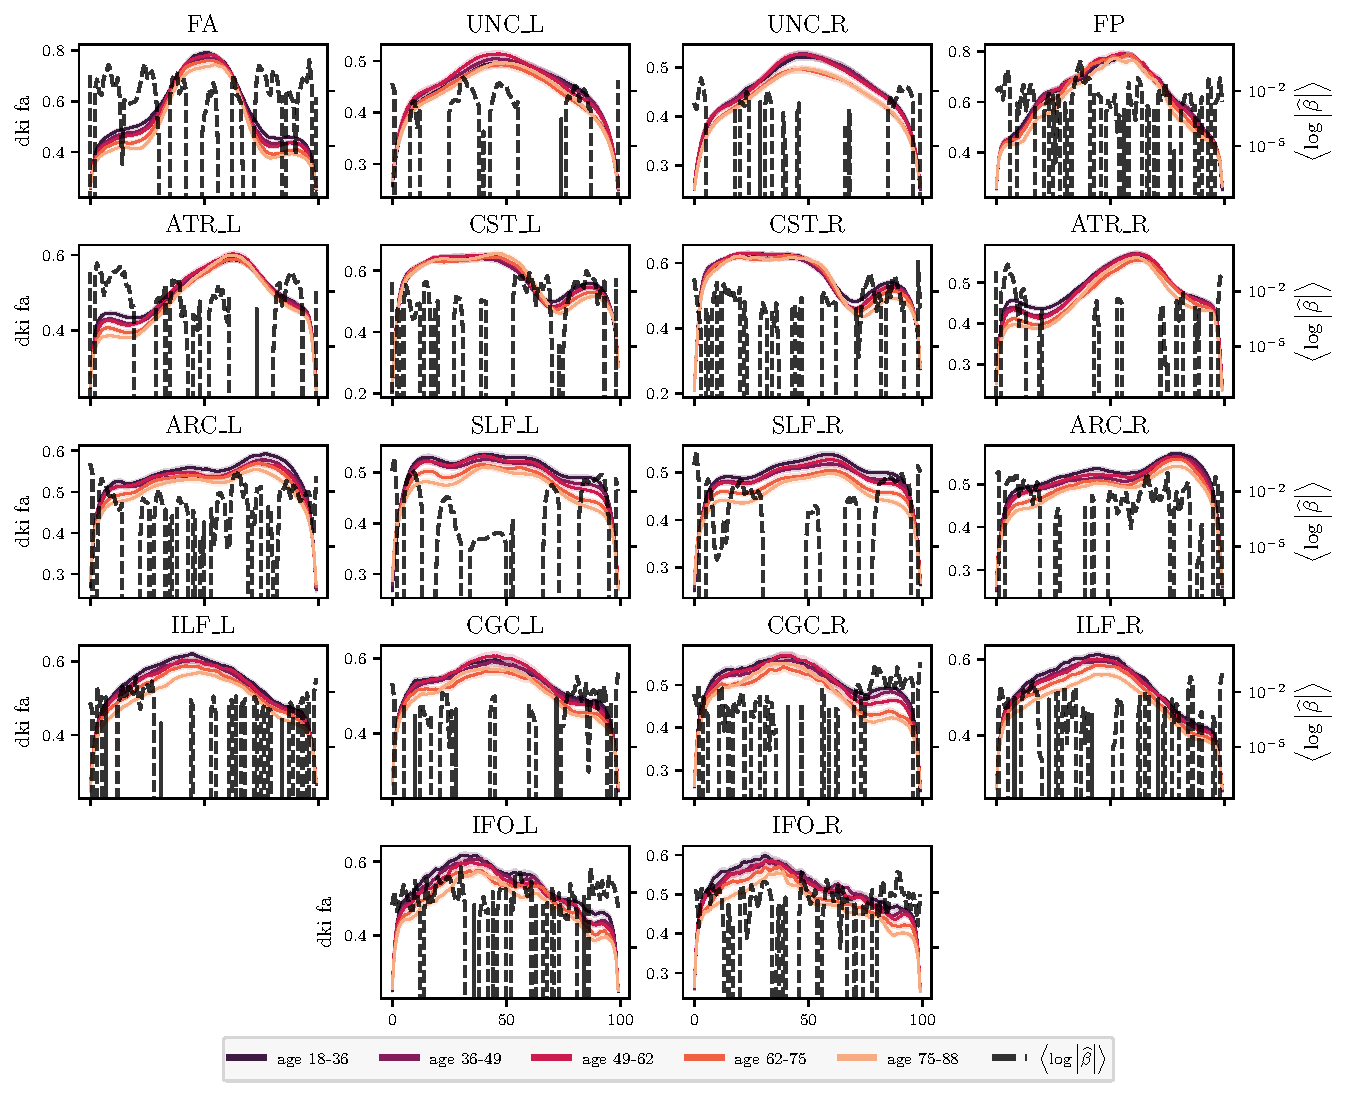
\includegraphics[width=\textwidth]{cc_coefs_profiles_fa.pdf}
    \caption{%
        {%
            \bf Fractional anisotropy (fa) bundle profiles and $\hat{\beta}$
            coefficients for age regression in the Cam-CAN dataset.
        }
        \label{fig:cc-bp:fa}
    }
\end{figure*}

\begin{figure*}
    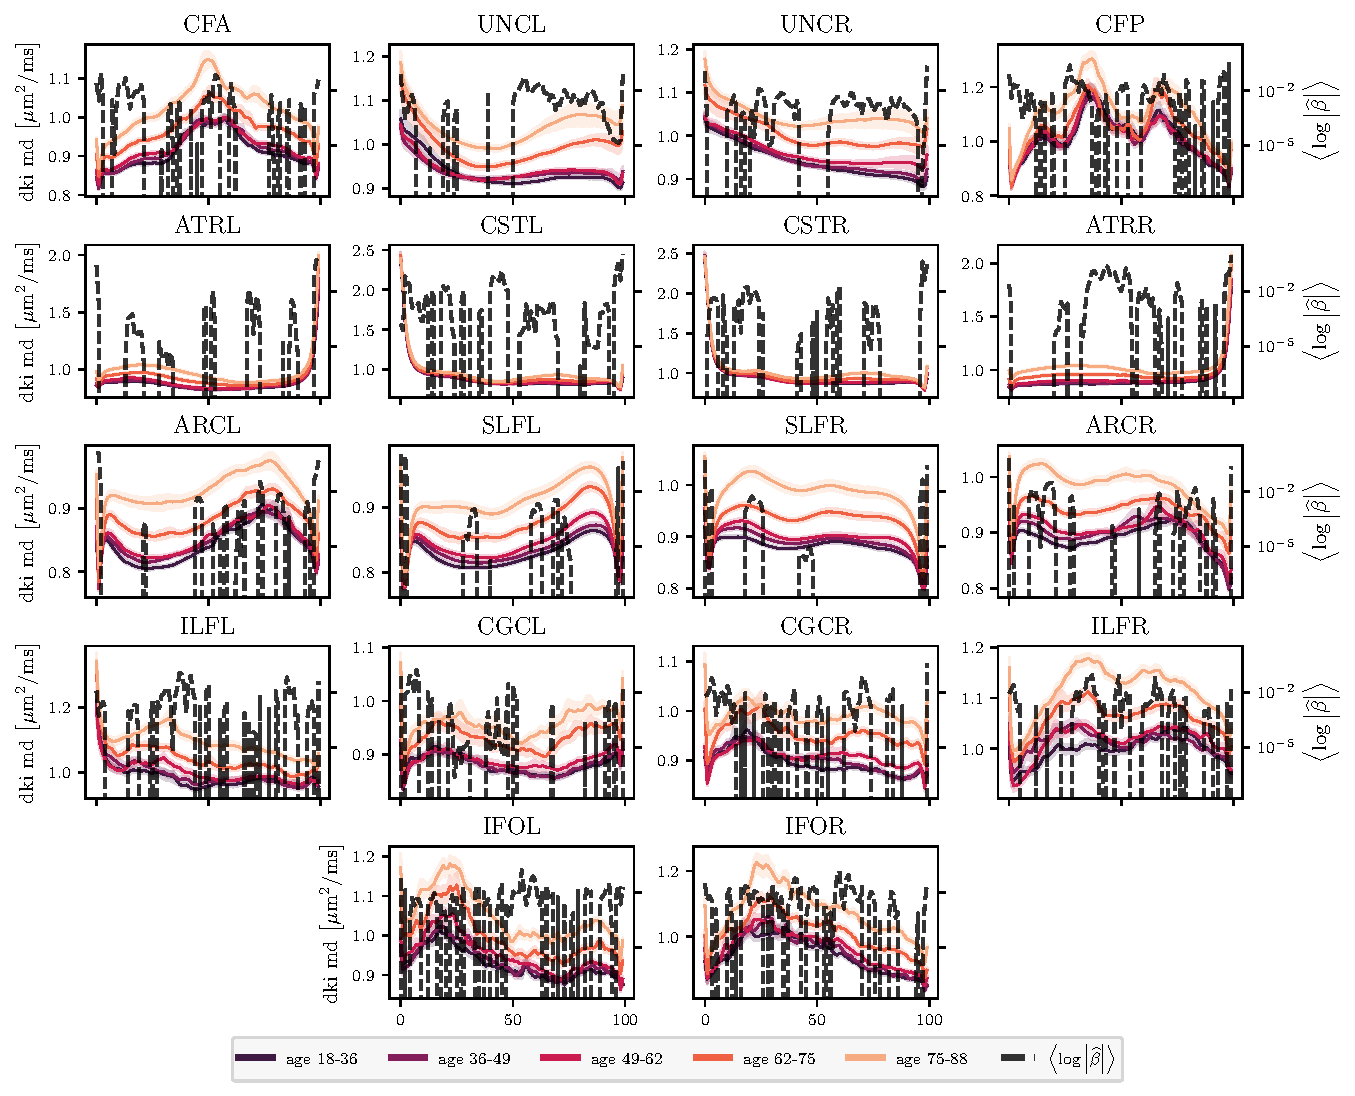
\includegraphics[width=\textwidth]{cc_coefs_profiles_md.pdf}
    \caption{%
        {%
            \bf Mean diffusivity (md) bundle profiles and $\hat{\beta}$
            coefficients for age regression in the Cam-CAN dataset.
        }
        \label{fig:cc-bp:md}
    }
\end{figure*}

\printfigures

\bibliographystyle{naturemag}
\bibliography{paper}

\end{document}

